\documentclass[11pt]{article}
\usepackage[margin=0.8in]{geometry}
\usepackage{amsmath,amssymb,graphicx,hyperref}
\setlength{\parindent}{0pt}\setlength{\parskip}{6pt}
\setlength{\emergencystretch}{3em}
\begin{document}
{\Large CRT reciprocity and the polynomial block radical}\\
November 13, 2026. Unsigned producer evidence [pcc:unverified].

\textbf{General component.} Over any field let $F,H$ be monic,
$a=\deg F$, $b=\deg H>0$, $b+1<a$, and suppose supplied polynomials obey
\[
 UF+V(fH)=1,\qquad \mu(Z)=[X^{a-1}]((ZV)\bmod F).
\]
For $\deg A\le a$, $\deg B\le b$, Lean characterizes the full block pairing:
\[
 \mu(AQ-fBT)=0\quad\text{for all }\deg Q\le a,\ \deg T\le b
 \quad\Longleftrightarrow\quad (A,B)=(cF,dH)
\]
for scalars $c,d$. This uses the actual quotient pairing, not a rank
assumption. No characteristic or separability condition is imposed.
The even norm chart $a=b+2$ fits; constant $H$ is excluded here.

\textbf{Core proof.} Bounded CRT remainders satisfy $SH+TF=P$:
the difference is divisible by $FH$ but has smaller degree. Comparing the
top coefficient gives reciprocity. The weighted instance is
\[
 \mu(fR)+[X^{b-1}]((RU)\bmod H)=0,\qquad \deg R<a+b-1.
\]
The existing coefficient detector shows that a unit-weighted quotient pairing
annihilates $P$ exactly when its modulus divides $P$. At the bounded degree,
this is exactly scalar span. Applying this separately to the upper and lower
blocks gives the displayed radical. For full lower tests,
$\deg(BT)\le2b<a+b-1$ explains the strict gap.

\begin{center}
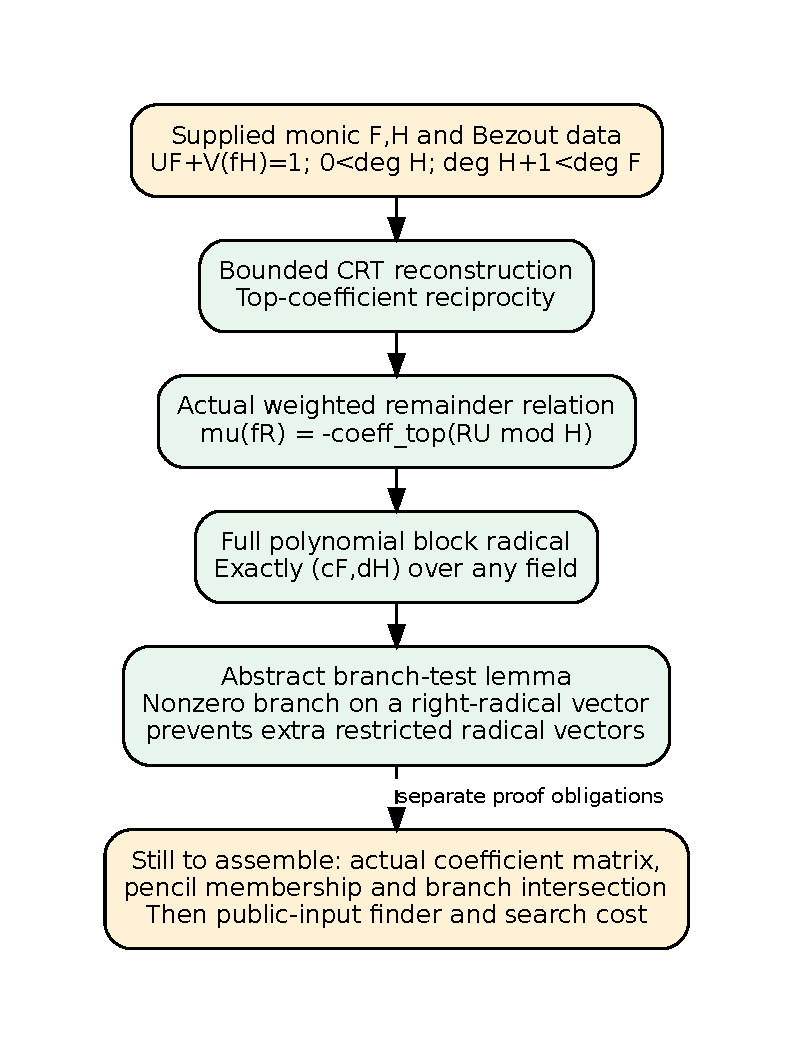
\includegraphics[width=0.9\linewidth,height=0.39\textheight,keepaspectratio]{bridge.pdf}
\end{center}

\newpage
{\Large Branch restriction, evidence and remaining assembly}

\textbf{Branch-test component.} For a bilinear pairing $\mathcal B$ and
linear functional $\ell$, suppose $k$ is in the right radical and
$\ell(k)\ne0$. Then vanishing against all tests in $\ker\ell$ is equivalent
to vanishing against all tests. Indeed every $v$ can be replaced by
$v-\ell(v)\ell(k)^{-1}k$. This proves no new left-radical vectors arise
under that explicit condition. Identifying the actual polynomial branch,
its scalar intersection and coefficient matrix remains an assembly task.

\textbf{Proof map.} \path{NormCRTReciprocity} supplies reconstruction,
coefficient comparison, canonical remainders and weighted reciprocity.
\path{NormPairingRadical} supplies ideal annihilators, bounded/full upper and
lower radicals, \path{normBlockRadical} and \path{branchTestsDetectFull}.
Exact hypotheses, fourteen unsigned claim bindings, sources and raw receipts
are linked from the accompanying Markdown report.

\textbf{Checks.} Lean4.35.0 with unchanged pinned CryptoLean/Mathlib.
Frozen source commits \path{3487f067d} (CRT) and \path{0d1208d8b} (radical).
The first gate covers95 declarations before the radical module was tracked;
the final gate covers104 with zero failing and zero trusted declarations.
Both import-inclusive fresh replays exited0; their separate statuses are retained.
Only standard foundations \path{propext}, \path{Classical.choice} and
\path{Quot.sound} are admitted. No signed PCC verdict is claimed.
The first radical build failed on an overbroad rewrite; subsequent builds
correct it. Failed and completed logs are preserved separately.

Native record \path{IDC1h4b52a3733d292783} checks the universal residual
\[
 (PV-FQ)H+(PU-HT)F-P=P(UF+VH-1)-FH(Q+T).
\]
The unchanged issuer/checker uses 32 statement-derived and 32 extra-stream
points, with exact universal proof-source hash. It does not execute Lean or
establish conditional degree or radical conclusions. Adapter tests:22 pass,
including inherited tamper/statement-swapping controls. No timing claim.

\textbf{Relation to rank-directed completion.} The earlier proposal sought
$W_{\rm new}=W_{\rm base}+C(T)H(T)$ with reduced crossing rank. Quotient
moments give a concrete alternative form with a characterized radical.
Reachability through that completion family and an efficient choice of its
free coefficients are not established by these results.

\textbf{Next obligations.} Identify actual bounded coefficient matrices,
normalization factors, $\mu(G)=0$ and coefficient-pencil membership; instantiate
the branch lemma and corank1 recovery; cover degree drops. Then construct
moments from public data with accounted $2^{o(n)}$ bit cost,
$n=\lceil\log_2r\rceil$. Current B\'ezout data is supplied with the witness.

\textbf{Sources and resources.} Exact pinned Mathlib monic-division,
coefficient, degree and coprime declarations; previous detector and next-proof
note. KB unavailable; bounded review, no priority claim for classical CRT.
No paid job, empirical timing/scaling campaign, benchmark or ecdb update.
Monthly isolab budget remains exhausted. Editable DOT/SVG/PDF diagram and
source-linked Markdown report accompany this PDF.
\end{document}
